\documentclass[12pt]{article}
\usepackage{geometry}                % See geometry.pdf to learn the layout options. There are lots.
\geometry{letterpaper}                   % ... or a4paper or a5paper or ... 
%\geometry{landscape}                % Activate for for rotated page geometry
\usepackage[parfill]{parskip}    % Activate to begin paragraphs with an empty line rather than an indent
\usepackage{daves,fancyhdr,natbib,graphicx,dcolumn,amsmath,lastpage,url}
\usepackage{amsmath,amssymb,epstopdf,longtable}
\usepackage{paralist}  % need to properly formulate standard answer blocks
\usepackage[final]{pdfpages}
\DeclareGraphicsRule{.tif}{png}{.png}{`convert #1 `dirname #1`/`basename #1 .tif`.png}
\pagestyle{fancy}
\lhead{CE 3305 Fluid Mechanics; Exercise Set 11}
\rhead{Name:\_\_\_\_\_\_\_\_\_\_\_\_\_\_\_\_\_\_\_\_\_\_\_\_\_\_\_\_\_\_\_\_\_\_}
\lfoot{REVISION A}
\cfoot{}
\rfoot{Page \thepage\ of \pageref{LastPage}}
\renewcommand\headrulewidth{0pt}
%%%%%%%%%%%%%%%%%%%%%%%%%%%%%%%%%%%%
\begin{document}
%%%%%%%%%%%%%%%%%%%%%%%%%%%%%%%%%%%
\begingroup
\begin{center}
{\textbf{{ CE 3305 Engineering Fluid Mechanics} \\ Exercise Set 11 \\ Summer 2018 -- GERMANY} }
\end{center}
\endgroup
\begingroup
~\newline
\textbf{Purpose} :  Application of Conservation of Mass for a System \\
\textbf{Assessment Criteria} : Completion, plausible solutions, use \textbf{R} as a calculator. \\~\\
\textbf{Exercises}

\begin{enumerate}
\item (Problem 5.32 pg 198)  Figure \ref{fig:HeatExchange} is a cross section of a heat exchanger comprised of three circular pipes housed inside a larger circular pipe.  
The internal diameter of the three smaller pipes is 2.5 $cm$ and the pipe wall thickness is 3 $mm$.  The inside diameter of the larger pipe is 8 $cm$.  If the velocity of the fluid in the region between the smaller pipes and the larger pipe is 10 $m/s$, what is the discharge in $m^3/s$?  

\begin{figure}[h!] %  figure placement: here, top, bottom, or page
   \centering
   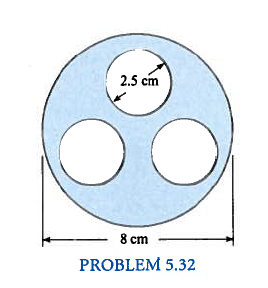
\includegraphics[width=2in]{HeatExchange.jpg} 
   \caption{Cross-section of heat exchanger}
   \label{fig:HeatExchange}
\end{figure}

\clearpage
\item (Problem 5.55 pg 200) Figure \ref{fig:TwoHoleTank} is a schematic a tank with a drain in the bottom that has cross-sectional area of 0.0025 $m^2$ and an inlet line on the side with a cross-sectional area of 0.0025 $m^2$, as shown.  
The cross-sectional area of the tank is 0.1 $m^2$.  
The velocity of the liquid flowing out the bottom hole is $V = \sqrt{2~gh}$, where $h$ is the height of the water surface above the outlet.
At an instant in time, the water level in the tank is 1 $m$ and rising at the rate of 0.1 $cm/s$.  
The liquid is incompressible.
Find the velocity of the liquid through the inlet.

\begin{figure}[h!] %  figure placement: here, top, bottom, or page
   \centering
   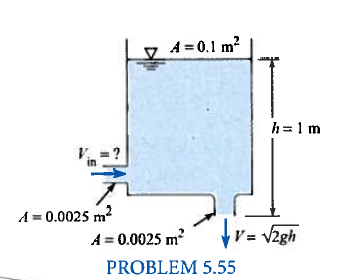
\includegraphics[width=3.5in]{TwoHoleTank.jpg} 
   \caption{Surge tank with two inlet/outlet connections.}
   \label{fig:TwoHoleTank}
\end{figure}

\end{enumerate}
\end{document}  